% 等离子体基础第二次作业

\section{等离子体基础第二次作业}

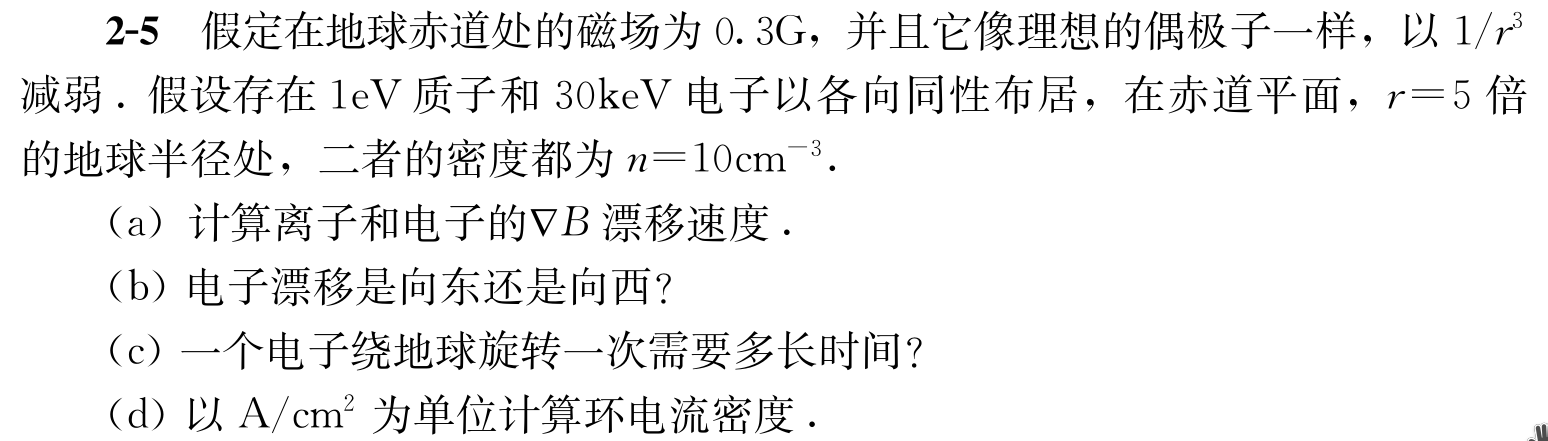
\includegraphics[width=0.9\textwidth]{figures/2022-09-30T114621+0800.png}

\subsection{Solution to 2-5}
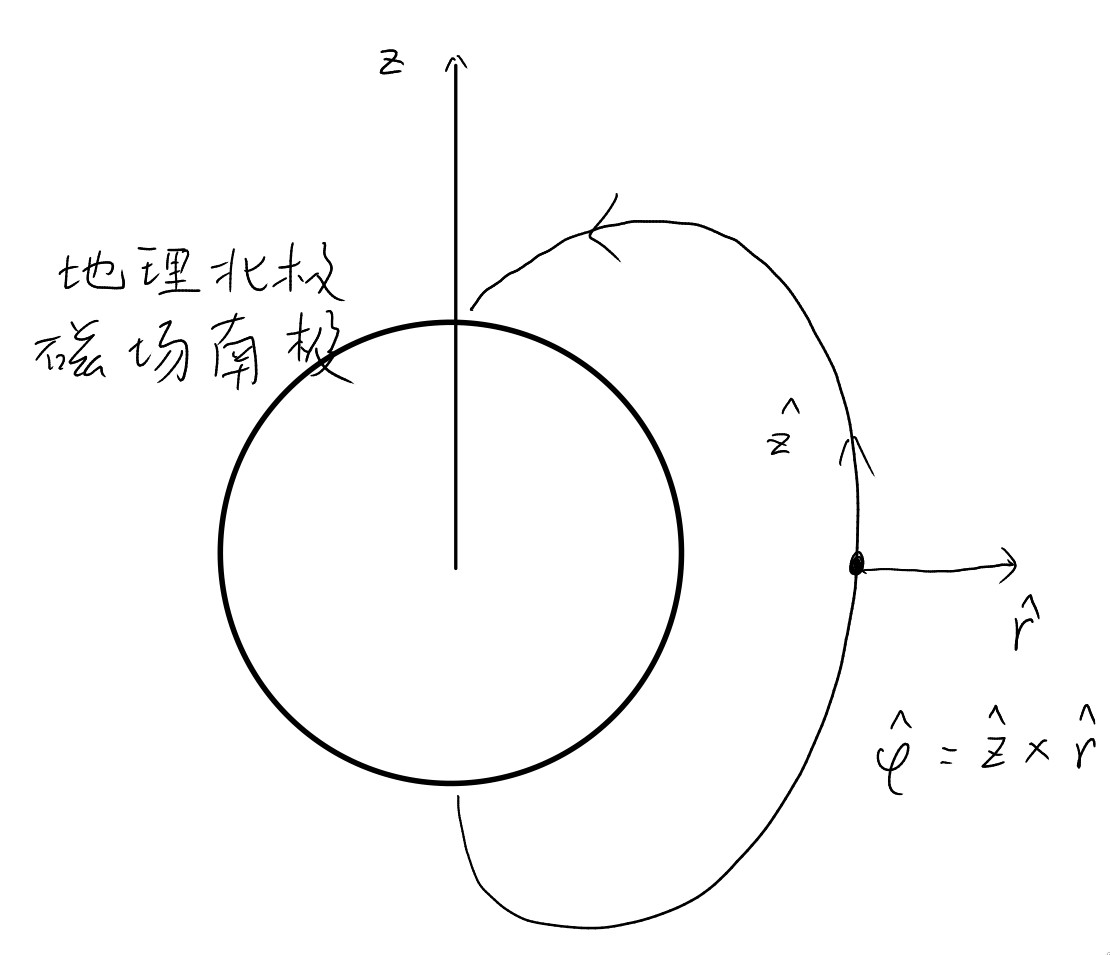
\includegraphics[width=0.5\textwidth]{figures/2022-09-30T114803+0800.png} \\

\noindent \textbf{(a)} 
如图所示,粒子垂直于磁场方向的速度\(v_{\perp}\)有两个自由度构成,
\begin{equation}
  \frac{1}{2} m v_\perp^2 = \frac{i}{2}kT = k_BT
\end{equation}
将质子的漂移速度\(\vb{v}_{\grad B}\)记为\(\vb{v}_p\),
将电子的漂移速度\(\vb{v}_{\grad B}\)记为\(\vb{v}_e\),
根据书本的式(2-24)
\begin{equation}
  \vb{v}_{\grad B} = \pm \frac{1}{2} v_{\perp} r_L \frac{\vb{B} \cross \grad B}{B^2}
  \label{eq:v}
\end{equation}
其中 Larmor radius 为
\begin{equation}
  r_L = \frac{m v_\perp c}{\abs{q} B_G}
\end{equation}
设地球赤道处的磁场\(B_0 = B(r_0) = 0.3 \si{G}\),则磁感应强度方向沿着\(\vu{z}\)方向,
表达式为
\begin{equation}
  \vb{B} = \frac{B_0 r_0^3}{r^3}  \vu{z}= \frac{K}{r^3} \vu{z}
\end{equation}
磁场大小梯度
\begin{equation}
  \grad B = \pdv{B}{r} \vu{r} = -\frac{3 K}{r^4} \vu{r}
\end{equation}
带入式~\eqref{eq:v} 可得电子漂移速度
\begin{equation}
  \begin{aligned}
    \vb{v}_e &= - \eval{\frac{1}{2} v_{\perp} r_L \frac{\vb{B} \cross \grad B}{B}}_{r=5r_0}\\
             &= \eval{\frac{3}{2} \frac{m_e v_\perp^2 cr^2}{q K}  \vu{\phi}}_{r=5 r_0} \\
             &= \eval{ \frac{3 k_B T_e cr^2}{q K}  \vu{\phi}}_{r=5 r_0} \\
             &= 25 \times \frac{3 k_B T_e c}{q B_0 r_0}  \vu{\phi} \\
             &= \SI{1.17e8}{cm / s}
  \end{aligned}
\end{equation}
质子漂移速度
\begin{equation}
  \begin{aligned}
    \vb{v}_p &= \eval{\frac{1}{2} v_{\perp} r_L \frac{\vb{B} \cross \grad B}{B}}_{r=5r_0}\\
             &= -\eval{\frac{3}{2} \frac{m_p v_\perp^2 c r^2 }{q K} \vu{\phi}}_{r=5 r_0} \\
             &= -\eval{\frac{3 k_B T_p c r^2 }{q K} \vu{\phi}}_{r=5 r_0} \\
             &= -25\times \frac{3 k_B T_p c }{q B_0 r_0} \vu{\phi} \\
             &= \SI{3906.25}{cm / s}
  \end{aligned}
\end{equation}

\noindent \textbf{(b)} 电子漂移向东。

\noindent \textbf{(c)}
\begin{equation}
    \Delta \tau = 
  \eval{\frac{2 \pi r}{v_e}}_{r=5 r_0} = 343.15s
\end{equation}

\noindent \textbf{(d)}
\begin{equation}
    \vb{J} = \vb{J}_p + \vb{J}_e = ne(\vb{v}_p - \vb{v}_e) = \SI{1.87e-10}{A/cm^2}
\end{equation}


%%% vim: set ts=2 sts=2 sw=2 isk+=\: et cc=+1 formatoptions+=mM:
